%% 
%% Copyright 2007-2025 Elsevier Ltd
%% 
%% This file is part of the 'Elsarticle Bundle'.
%% ---------------------------------------------
%% 
%% It may be distributed under the conditions of the LaTeX Project Public
%% License, either version 1.3 of this license or (at your option) any
%% later version.  The latest version of this license is in
%%    http://www.latex-project.org/lppl.txt
%% and version 1.3 or later is part of all distributions of LaTeX
%% version 1999/12/01 or later.
%% 
%% The list of all files belonging to the 'Elsarticle Bundle' is
%% given in the file `manifest.txt'.
%% 
%% Template article for Elsevier's document class `elsarticle'
%% with numbered style bibliographic references
%% SP 2008/03/01
%% $Id: elsarticle-template-num.tex 272 2025-01-09 17:36:26Z rishi $
%%
\documentclass[preprint,12pt]{elsarticle}


%% Use the option review to obtain double line spacing
%% \documentclass[authoryear,preprint,review,12pt]{elsarticle}

%% Use the options 1p,twocolumn; 3p; 3p,twocolumn; 5p; or 5p,twocolumn
%% for a journal layout:
%% \documentclass[final,1p,times]{elsarticle}
%% \documentclass[final,1p,times,twocolumn]{elsarticle}
%% \documentclass[final,3p,times]{elsarticle}
%% \documentclass[final,3p,times,twocolumn]{elsarticle}
%% \documentclass[final,5p,times]{elsarticle}
%% \documentclass[final,5p,times,twocolumn]{elsarticle}

%% For including figures, graphicx.sty has been loaded in
%% elsarticle.cls. If you prefer to use the old commands
%% please give \usepackage{epsfig}

%% The amssymb package provides various useful mathematical symbols
\usepackage{amssymb}
%% The amsmath package provides various useful equation environments.
\usepackage{amsmath}
%% The amsthm package provides extended theorem environments
%% \usepackage{amsthm}

%% The lineno packages adds line numbers. Start line numbering with
%% \begin{linenumbers}, end it with \end{linenumbers}. Or switch it on
%% for the whole article with \linenumbers.
%% \usepackage{lineno}
\usepackage{amssymb}   % For mathematical symbols
\usepackage{amsmath}   % For advanced math formatting
\usepackage{graphicx}  % For including images
\usepackage{hyperref}  % For clickable references and links


\journal{Finance Research Letters}

\begin{document}

\begin{frontmatter}

%% Title, authors and addresses

%% use the tnoteref command within \title for footnotes;
%% use the tnotetext command for theassociated footnote;
%% use the fnref command within \author or \affiliation for footnotes;
%% use the fntext command for theassociated footnote;
%% use the corref command within \author for corresponding author footnotes;
%% use the cortext command for theassociated footnote;
%% use the ead command for the email address,
%% and the form \ead[url] for the home page:
\title{Unleashing the Power of Deep Learning: A Performance Comparison of LSTM, GRU, and Transformer Models\tnoteref{label1}}
%% \tnotetext[label1]{}
%% \author{Name\corref{cor1}\fnref{label2}}
%% \ead{email address}
%% \ead[url]{home page}
%% \fntext[label2]{}
%% \cortext[cor1]{}
%% \affiliation{organization={},
%%             addressline={},
%%             city={},
%%             postcode={},
%%             state={},
%%             country={}}
%% \fntext[label3]{}

\title{}

%% use optional labels to link authors explicitly to addresses:
%% \author[label1,label2]{}
%% \affiliation[label1]{organization={},
%%             addressline={},
%%             city={},
%%             postcode={},
%%             state={},
%%             country={}}
%%
%% \affiliation[label2]{organization={},
%%             addressline={},
%%             city={},
%%             postcode={},
%%             state={},
%%             country={}}

%% Author names and affiliations
\author[label1]{Jagdish Chakole\corref{cor1}\fnref{}}
\ead{jchakole@iiitn.ac.in}

\author[label2]{Muktinath Vishwakarma}
\ead{author2@example.com}

\author[label1]{Nachiket N Doddamani}
\ead{nachiketdoddamani@gmail.com}

\author[label2]{Manish Kurhekar}
\ead{manishkurhekar@cse.vnit.ac.in}

%% Corresponding author footnote
\cortext[cor1]{Corresponding author}

%% Footnotes for additional information
%%\fntext[fn1]{Jagdish Chakole is supported by XYZ grant/project.}

%% Affiliations
\affiliation[label1]{
	organization={Indian Institute of Information Technology Nagpur}, % Department and Organization
	addressline={}
	city={}
	postcode={441108}, 
	state={Maharashtra},
	country={India}
}

\affiliation[label2]{
	organization={Visvesvaraya National Institute of Technology Nagpur}, % Department and Organization
	addressline={}
	city={}
	postcode={440010}, 
	state={Maharashtra},
	country={India}
}

\author{}

%% Abstract
\begin{abstract}
Metals, particularly non-ferrous metals, play a pivotal role as raw materials in numerous industries, serving as essential components for a nation's industrial and economic growth. The fluctuating prices of these metals pose a significant challenge for industries aiming to procure them at optimal costs. While various approaches, including machine learning, have been employed for metal price prediction, there remains room for improvement in the accuracy and efficiency of these models. Notably, recent advancements in deep learning have demonstrated impressive performance. This research delves into the application of state-of-the-art deep learning models tailored for sequential data to enhance the prediction accuracy of non-ferrous metal prices. The main contribution of this research work is the use of the Transformer model to develop a predictive model to predict the non-ferrous metal price and its comparison with the state-of-the-art deep learning models tailored for sequential data.  Through empirical studies, we explore the efficacy of prominent deep learning architectures,
including Long Short-Term Memory (LSTM), Gated Recurrent Unit (GRU), and Transformer models. The objective is to discern the model that exhibits superior performance in capturing the intricate patterns and temporal dynamics inherent in metal price time series data. Our experimental results show that the proposed Transformer-based model outperformed the LSTM, and GRU-based models to predict non-ferrous metal prices including Aluminium, Copper, Zinc, and Nickel.
\end{abstract}

%%Graphical abstract
%%\begin{graphicalabstract}
%\includegraphics{grabs}
%%\end{graphicalabstract}
%%Research highlights
\begin{highlights}
\item Research highlight 11
\item Research highlight 2
\end{highlights}

%% Keywords
\begin{keyword}
%% keywords here, in the form: keyword \sep keyword

%% PACS codes here, in the form: \PACS code \sep code

%% MSC codes here, in the form: \MSC code \sep code
%% or \MSC[2008] code \sep code (2000 is the default)

\end{keyword}

\end{frontmatter}

%% Add \usepackage{lineno} before \begin{document} and uncomment 
%% following line to enable line numbers
%% \linenumbers

%% main text
%%

%% Use \section commands to start a section

\section{Introduction}
Metals are the basic raw materials for many industries. Many metals are used to manufacture machines for diverse sectors like agriculture, automobile, construction, and more. Almost all industries directly or indirectly depend upon metals. So, the price of the finished product depends on the metals, that are required as raw materials to a product or as raw materials to equipment required to manufacture the product. The price of the metals depends on many diverse factors including demand and supply of the metal, geopolitical situation, etc. The price of the metals fluctuates over time. One of the objectives of the industry is to purchase metals at an optimal price as the price of their finished product is based on raw materials price. Governments and industries are in need to know the future price of these metals for decision-making.
\par The motivation for this work is related to the advancement in computer technology and the Data Science domain and its ubiquitous use. The majority of the global stock and commodity exchanges are working online because of the technological advancements. Historical and current trading data like price action, and volume data is easily available at affordable cost in electronic form \cite{chakole2023tutorial}. The performance of data-driven machine learning and deep learning methods\cite{chakole2021convolutional} has improved significantly. The availability of models and clean datasets have the potential to predict future prices or trends.
\par In this research work, we are interested in predicting the future price of non-ferrous metals as it is significant for the growth and development of the country. We are specifically interested in non-ferrous metals, as these metals are mostly useful in manufacturing industries because of their significant properties \cite{watkins2004econometric}. Non-ferrous metals are non-magnetic and non-iron based metals like Aluminium, Copper, Zinc, Nickel, etc.
\par This research makes two significant contributions. Firstly, it introduces a novel model leveraging the Transformer architecture for predicting metal prices, marking a departure from conventional approaches. Notably, prior studies have not explored the application of Transformer models for forecasting non-ferrous metal prices. Secondly, the study conducts a comprehensive performance comparison between the proposed Transformer-based model and a state-of-the-art deep learning model designed for analyzing sequential data.
\par The time series dataset for the daily prices of non-ferrous metals exhibits a consistent time difference between consecutive data points, rendering it a sequential data format. Similarly, Natural Language Processing (NLP) data also follows a sequential structure. Recently, there has been a notable surge in the development of deep learning-based predictive models for sequential data within the NLP domain, demonstrating noteworthy performance. This research delves into the application of such models for predicting metal prices.
\par The London Metal Exchange (LME) stands as a prominent global platform facilitating the trade of metals. The pricing dynamics of numerous metals, particularly non-ferrous ones, are internationally influenced by the LME. Hence, the dataset sourced from the LME serves as the foundation for our research endeavors.
\par The rest of the paper is organized as Section 2 covers the motivation and background that discusses the various approaches and methods used to date to predict metal prices. Section 3 discusses the method used in this research work. The Transformer-based architecture of the proposed system is discussed in Section 4. In Section 5, we discuss the experimental dataset and performance evaluation measures used in this research work. The experimental results and their significance are discussed in Section 6. Section 7 concludes the paper.


\section{Motivation and Background}


In the subsequent section, we explore previous research endeavors focusing on forecasting metal prices conducted by various scholars. Kriechbaumer et al. \cite{kriechbaumer2014improved} introduced an enhanced forecasting methodology for non-ferrous metal prices utilizing a Wavelet-ARIMA model. This model dissects the price time series into frequency and time domains, thereby refining forecasting precision. In another study, Kristjanpoller et al. \cite{kristjanpoller2017volatility} proposed a hybrid model integrating Artificial Neural Networks (ANN) and the Generalized Autoregressive Conditional Heteroskedasticity (GARCH) model to predict the volatility of copper, gold, and silver. Concerning short-term gold price prediction, Hajek et al. \cite{hajek2022fuzzy} introduced a fuzzy rule-based system incorporating financial price data and news sentiment data for training. They argue that news data is more relevant for predicting prices one day ahead, while historical trading data gains significance for forecasting prices five days in advance. Guha et al. \cite{guha2016gold} employed the ARIMA model to forecast future gold prices in the Indian stock market using price series data. Additionally, Zhichao He et al. \cite{he2023novel} proposed a hybrid forecasting model for non-ferrous metal prices. Their approach entails decomposing the price series into multiple subseries, utilizing the ARIMA model for forecasting low-frequency subseries, and subsequently aggregating them to reconstruct the original series. Notably, the authors underscored the optimal utilization of residual values from the series for effective forecasting.
\par Zhou et al. \cite{zhou2019precious} predicted the prices of gold and palladium using the Deep Regularization Self-Attention Regression model, incorporating components such as CNN, LSTM, and self-attention. Their approach involved extracting spatial features through CNN and temporal features via LSTM. This model outperformed the ARIMA, SVR, CNN, and LSTM models. Addressing the instability of raw single series price data on the LME, Liu et al. \cite{liu2020non} decomposed the data using variational mode decomposition into subseries, employing LSTM for forecasting each subseries and aggregating them with an aggregation function. Astudillo et al. \cite{astudillo2020copper} utilized support vector regression to forecast copper prices for the next 5 and 10 days, achieving an RMS of $\leq$ 2.2\% in their experimentation with London Metal Exchange data. Li et al. \cite{li2023novel} proposed a model based on LSTM and Multivariate Mode Decomposition for metal price prediction, arguing that fusion models based on decomposition outperform single models.
\par Artificial Neural Network-based framework used in M{\'e}ndez-Su{\'a}rez et al.\cite{mendez2019artificial} to predict copper price five days ahead based on the current price data. Shao et al. \cite{shao2019nickel} optimized the parameters of the LSTM model using improved particle swarm optimization to predict the nickel price. The experimental results concluded that the proposed model outperformed the conventional LSTM and ARIMA. The EWT-GBDT model, combining Empirical Wavelet Transform (EWT) and Gradient Boosting Decision Trees, was introduced in the work by Gu et al. \cite{gu2021forecasting}. This model aimed to forecast the future price of nickel on the London Metal Exchange. The process involves selecting input features based on their correlation with the nickel price and subsequently decomposing the chosen input feature series into subseries using EWT. The resulting decomposed features are then fed into the Gradient Boosting Decision Trees (GBDT) for the final price prediction. According to their experimental results, the proposed EWT-GBDT model demonstrated superior performance compared to both the standalone GBDT and Adaboost models. Also, Zhao et al.\cite{zhao2022risk}, used a decomposition-based model for prediction.
\par We can outline that researchers initially experimented with statistical models such as the ARIMA model, which later evolved into variants or combinations of these models for metal price prediction. Subsequently, some researchers delved into machine learning techniques, followed by deep learning methods tailored for sequential data analysis. In our study, we investigate the effectiveness of contemporary deep learning models for sequential data in predicting metal prices.
\par Researchers have explored the versatility of the Transformer across various domains, demonstrating its effectiveness in many cases. Motivated by these successes, this work aims to investigate the Transformer architecture's applicability in predicting non-ferrous metal prices. Dosovitskiy et al. \cite{dosovitskiy2020image} delved into the application of the Transformer architecture in computer vision, revealing that the Vision Transformer outperformed traditional convolutional network-based models. Furthermore, the object detection Transformer was employed in the study by Carion et al. \cite{carion2020end}. Additionally, Dong et al. \cite{dong2018speech} introduced the Speech-Transformer model for speech recognition tasks, while Payne et al. \cite{payne2019musenet} utilized the Transformer for generating musical compositions. In the medical domain, Valanarasu et al. \cite{valanarasu2021medical} leveraged the Transformer architecture for image segmentation tasks. These studies collectively highlight the broad spectrum of domains where the Transformer architecture has shown promising performance.

\section{Methodology}
The objective of this research work is to explore the capabilities of the Transformer for the prediction of the non-ferrous metal price. We have compared the performance of the proposed model with the classic deep learning methods for sequential data viz RNN, LSTM, and GRU. This section introduces the intuition and architectures of these methods.
\subsection{RNN}
A feedforward Artificial Neural Network (ANN) is suitable for data with spatial features but it is not suitable for data having temporal features i.e. sequential data. In sequential data, there is a dependency between data at time instant $t$ and at time instant $t-1$. The ANN is not able to handle this dependency as it treats every data point independently. Recurrent Neural Networks (RNN) is a variant of ANN to handle sequential data \cite{rumelhart1986learning}. As shown in Fig. \ref{figrnn1}, in RNN the hidden layers are treated as a state (hidden state). The hidden state at time step $t$ is based on the hidden state at time step $t-1$ and input data (features) at time instant $t$ as indicated in Equation \ref{e1}. A hidden state acts as a memory that stores information till the previous data point. The output of RNN at time $t$ is based on hidden state $h_t$ at time $t$ as shown in Equation \ref{e2}.
\begin{equation} \label{e1}
	h_t = \tanh(x_{t},h_{t-1})\\
\end{equation}
\begin{equation}  \label{e2}
	O_t = f(h_{t})\\
\end{equation}

\begin{center}
	\begin{figure}[!htbp]
		\centering
		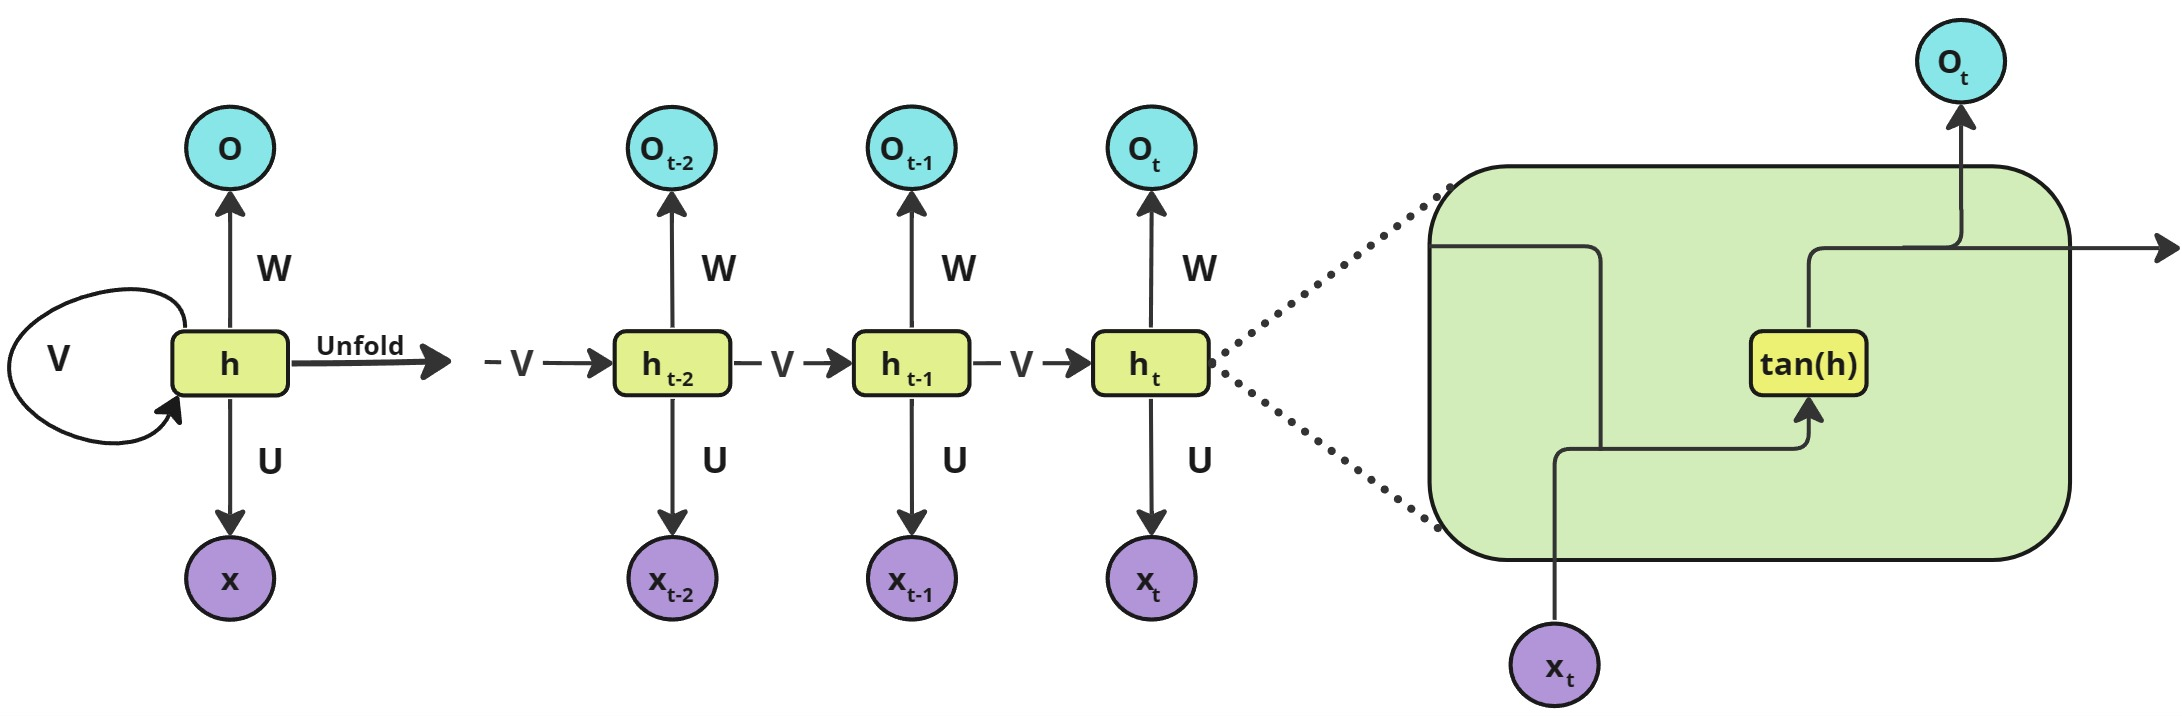
\includegraphics[width=15cm, height=7cm]{RNN.jpg}
		\caption{Recurrent Neural Network Architecture}
		\label{figrnn1}
	\end{figure}
\end{center}


Fig. \ref{figrnn1}, shows hidden states of RNN at different time instances. These different time instances share the same parameters. The RNN is capable of handling data dependencies in the sequential data but has some issues like it may have a Vanishing and Exploding gradient problem. The hidden state in RNN has limited capability so, it is not able to handle data dependencies if data is separated by many time steps.
\subsection{Long Short-Term Memory (LSTM)}
The RNN can handle the dependency between the data if the two relevant data points are not far apart but if there is a long-term dependency between data then the RNN suffers from vanishing gradient problem \cite{bengio1994learning}. The LSTM model is a variant of the RNN model and it can handle this long-term dependency problem \cite{hochreiter1997long}.
\par As shown in Fig. \ref{lstm1}, in addition to hidden state $h_t$ the LSTM has one more state called cell state $C_t$. The hidden state is short-term memory and the cell state is long-term memory. The cell state $C_t$ is like a convey belt that passes information from the current time step to the next time step. Unlike RNN the LSTM does not remember all previous information. It only remembers relevant information, passes only necessary information to the next time step, and takes only fruitful information from the input using three gates viz. forget gate, output gate, and input gate. In Fig. \ref{lstm1}, The forget gate $f_t$ govern by the following equation, decides which part of the input cell state $C_{t-1}$ is forgeted.
\begin{equation}
	\quad f_t = \sigma(W_{f} \cdot [h_{t-1},x_t] + b_{f})
\end{equation}
The input gate decides this part of the input added to the cell state $C_{t}$, govern by following equations as $i_t\ast \tilde{C_t}$.
\begin{equation}
	\quad i_t = \sigma(W_{i} \cdot [h_{t-1},x_t] + b_{i})
\end{equation}
\begin{equation}
	\quad \tilde{C_t}= \tanh(W_{c} \cdot [h_{t-1},x_t] + b_{c})
\end{equation}
The cell state ${C_t}$ is computed as 
\begin{equation}
	\quad {C_t}= f_t\ast {C_{t-1}} + i_t\ast \tilde{C_t}
\end{equation}
The output $h_t$ is computed as
\begin{equation}
	\quad {o_t}= \sigma(W_{o} \cdot [h_{t-1},x_t] + b_{o})
\end{equation}
\begin{equation}
	\quad {h_t}= {o_t}\ast  \tanh(C_t)
\end{equation}
In the above equations, $W$ is the weight vector and $b$ is the bais of the respective gate.



\begin{center}
	\begin{figure}[!htbp]
		\centering
		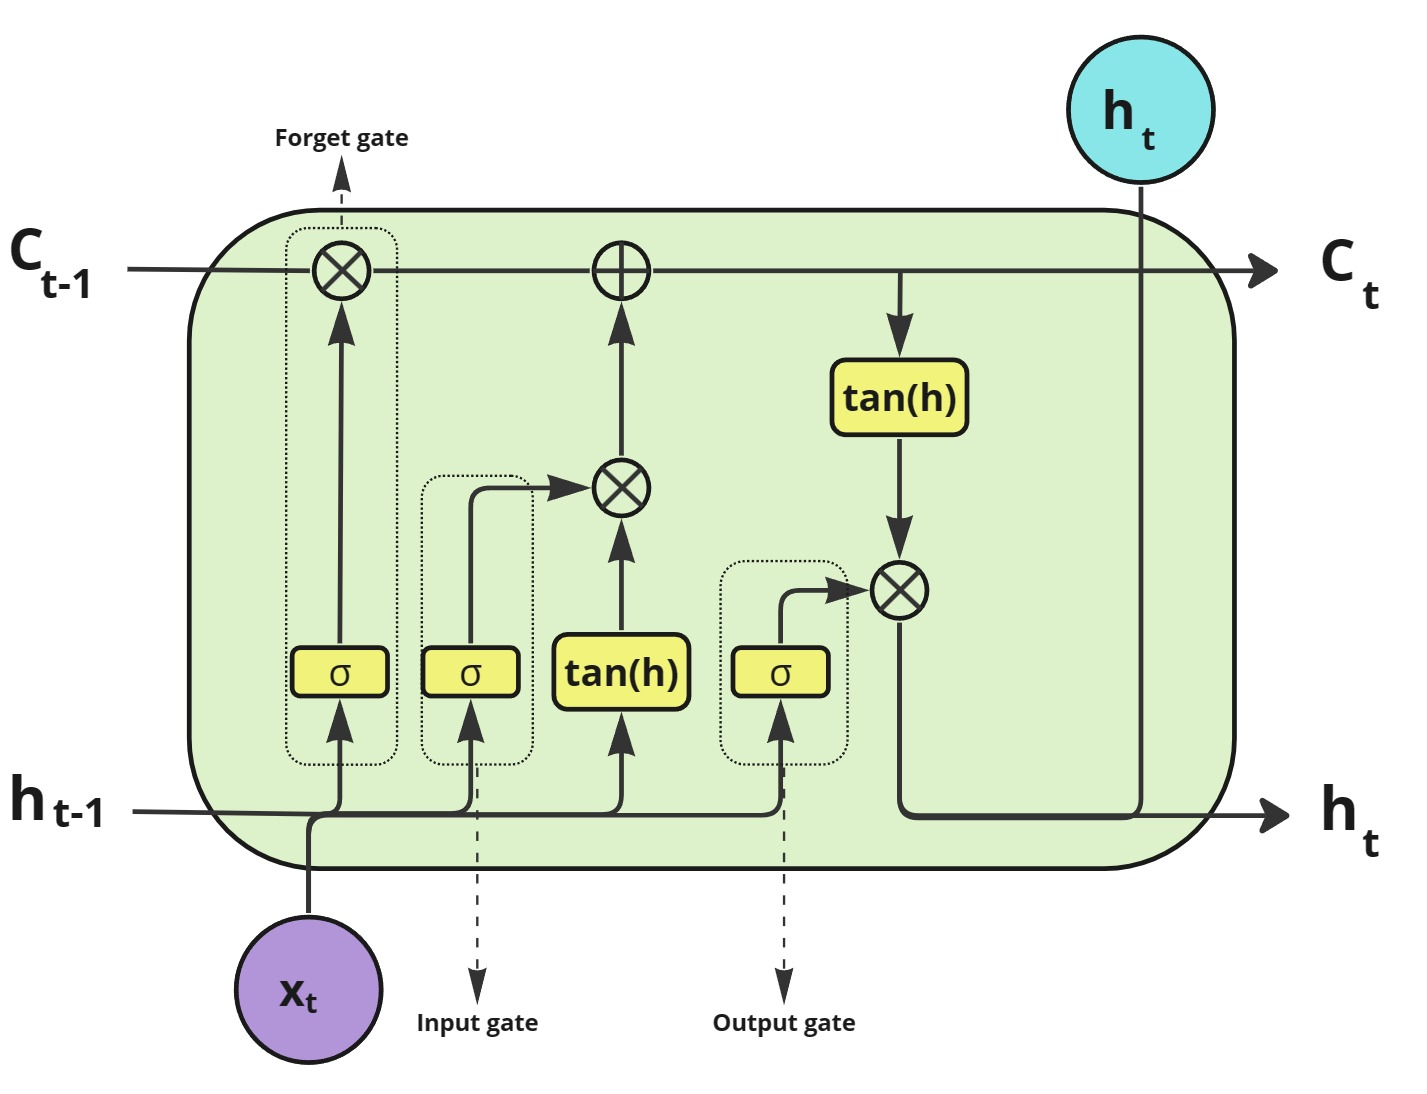
\includegraphics[width=10cm, height=8cm]{LSTM.jpg}
		\caption{LSTM architechture}
		\label{lstm1}
	\end{figure}
\end{center}


\subsection{GRU}
\par Gated Recurrent Unit (GRU) is introduced in \cite{cho2014learning}, like LSTM it is also a type of RNN that addresses the vanishing gradient problem. Like LSTM it also has gates but only two gates instead of three gates in LSTM. These two gates are namely the reset gate and the update gate as shown in Fig. \ref{gru}. Unlike LSTM there is only one state. It has only a hidden state no cell state. The GRU architecture is less complex compared to LSTM. It is computationally less complex compared to LSTM. LSTM can capture better long-term dependency. The reset gate equation is as follows. The vector $r_t$ depends on the previous hidden state $h_{t-1}$ and current input $x_t$
\begin{equation}
	\quad r_t = \sigma(W_{r} \cdot [h_{t-1},x_t] + b_{r})
\end{equation}
The update gate is as follows. 
\begin{equation}
	\quad u_t = \sigma(W_{u} \cdot [h_{t-1},x_t] + b_{u})
\end{equation} 
The equation for candidate hidden state $\tilde{h_t}$ is as follows. where $\odot$ is elementwise multiplication.  
\begin{equation}
	\quad \tilde{h_t}= \tanh(W_{h} \cdot [r_t\odot h_{t-1},x_t] + b_{h})
\end{equation}
The current hidden state ${h_t}$ is computed as follows.
\begin{equation}
	\quad {h_t}= (1-u_t) \odot h_{t-1} + u_t \odot \tilde{h_t}
\end{equation}

\begin{center}
	\begin{figure}[!htbp]
		\centering
		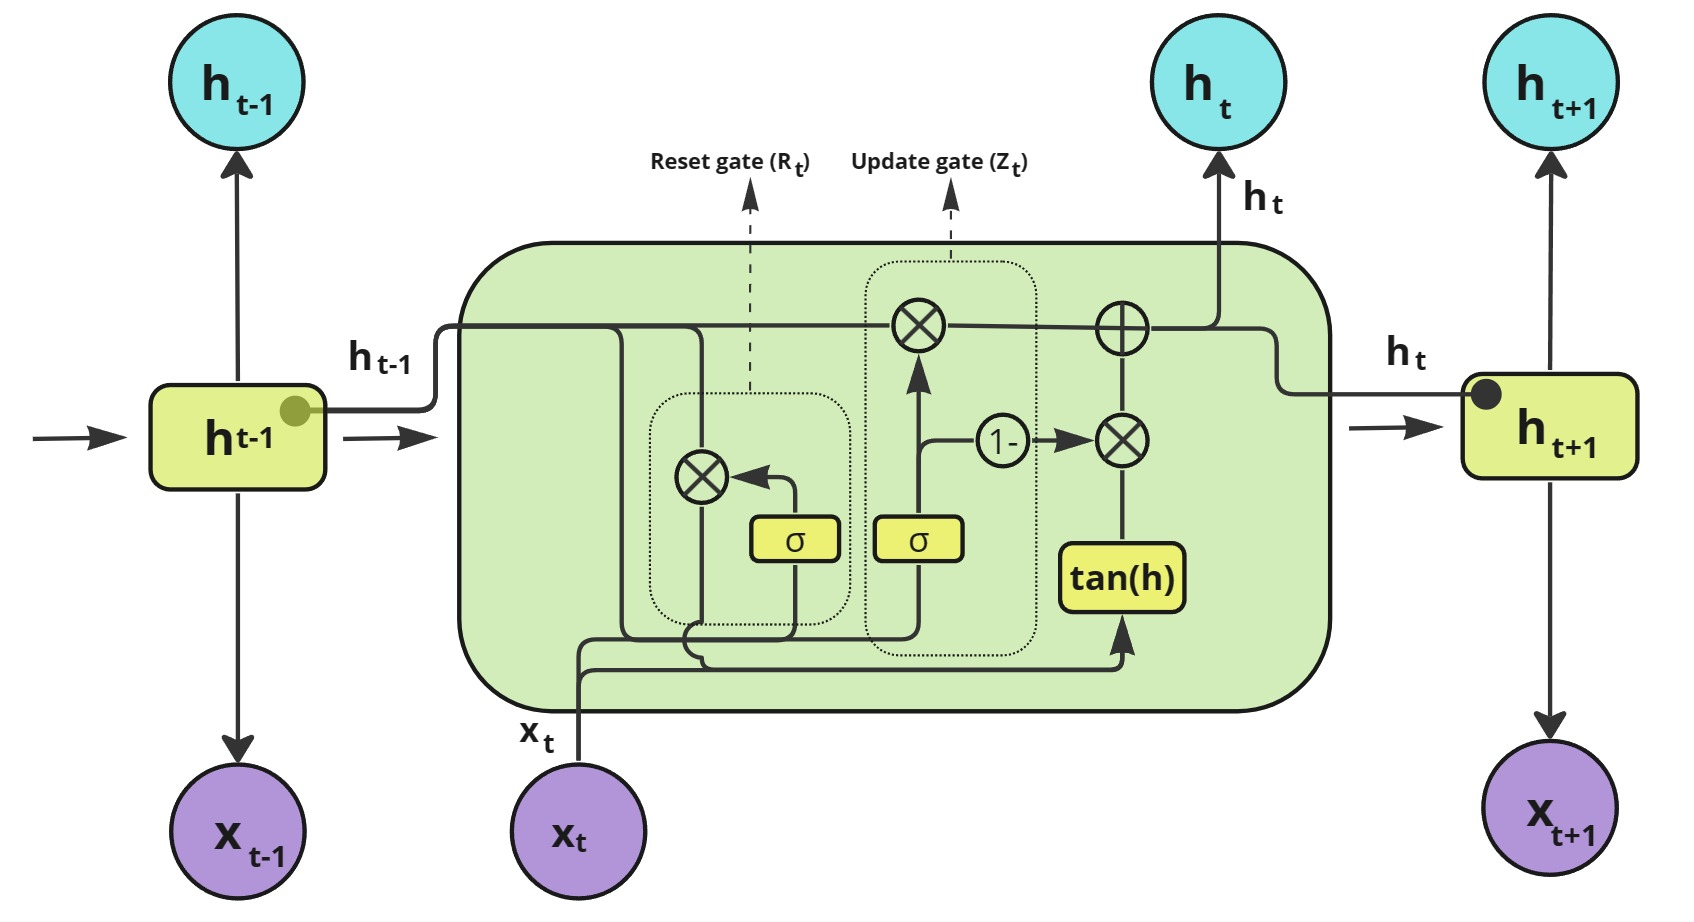
\includegraphics[width=11cm, height=7cm]{GRU.jpg}
		\caption{GRU architechture}
		\label{gru}
	\end{figure}
\end{center}

\subsection{Transformer}
Unlike LSTM, GRU, and other primitive RNN-based models that rely on sequential processing, the Transformer on the other hand adopts a localized and hierarchical processing approach inspired by Convolutional Neural Networks (CNN). The key innovation lies in the integration of attention-based mechanisms which allows parallel computation and makes it possible to capture long-range dependencies thereby making it more efficient as shown in Fig. \ref{transformer}.
\begin{center}
	\begin{figure}[!htbp]
		\centering
		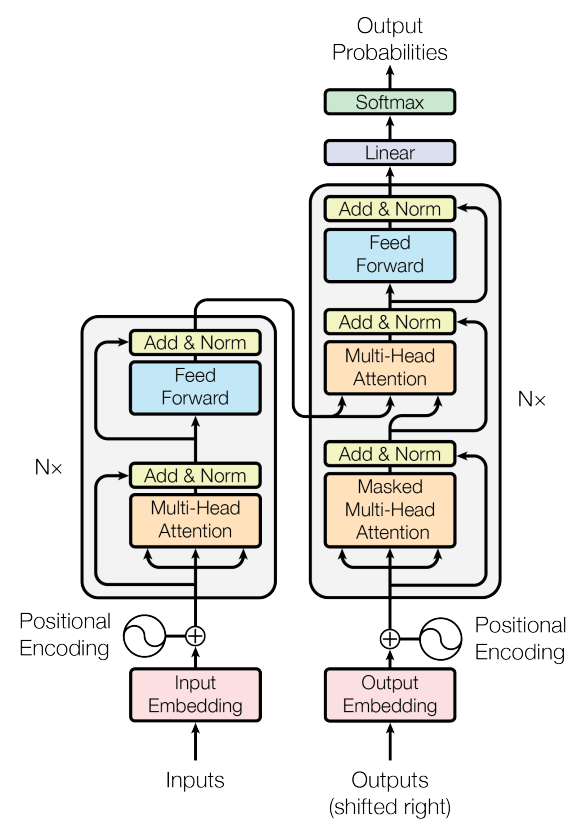
\includegraphics[width=10cm, height=12cm]{transformer.png}
		\caption{The Transformer - model architecture\cite{vaswani2017attention}}
		\label{transformer}
	\end{figure}
\end{center}
\begin{itemize}
	\item \textbf{Attention Mechanism}\\
	It is a mechanism that assigns different levels of importance to different parts of the input sequence, enabling the model to selectively focus on different parts of the input sequence when producing an output, thereby selecting the most relevant information \cite{bahdanau2014neural}. Attention mechanisms are classified into self-attention, multi-head attention, and local attention, each offering different benefits and trade-offs.
	
	\item \textbf{Transformer}\\
	Introduced in the paper \cite{vaswani2017attention}, Transformer architecture is the fundamental building block of Large Language Models (LLMs). The self-attention mechanism helps to capture long-distance context so that the sequence of the hidden states also attends to itself. A Transformer model can be classified into three categories: Encoders, Decoders, and Encoder-decoder models\cite{sutskever2014sequence}. The attention mechanism involves three sets of matrices: query(Q), key(K), and value(V). These matrices are derived from the input sequence.
	\begin{itemize}
		\item \textbf{Query (Q)}\\
		The query vector represents the element that is currently being focused on for the given context. In the context of self-attention mechanisms, it’s the vector of target input for which the attention weights are obtained. By utilizing the query matrix to alter the word representation, the system produces a query vector. This vector is then employed to compare against other words within the sentence.\\
		$q_{i}=W_{q}x_{i}$,  where $x_{i}$ represents the input query vector at position $i$, $q_{i}$ represents the projected query vector at position $i$,$W_{q}$ represents the weight matrix used for the query projection.
		\item \textbf{Value (V)}\\
		The system utilizes the key matrix to generate key vectors for every word present in the sentence. These key vectors are used in evaluating the relevance or similarity between the target word (using the query vector) and other words within the sentence. A greater similarity score between the query vector and a key vector signifies a more robust relationship between the respective words.\\
		$v_{i}=W_{v}x_{i}$
		\item \textbf{Key (K)}\\The value matrix produces value vectors for each word in the sentence. These vectors contain the contextual details of individual words. Following the computation of similarity scores using query and key vectors, the system proceeds to calculate a weighted sum of the value vectors. The weights assigned to each value vector are based on the similarity scores, thereby ensuring that the resulting contextual representation is predominantly influenced by relevant words.\\
		$k_{i}=W_{k}x_{i}$
		\item The encoding results in the word $C_i$, by applying attention mechanism to the projected vectors.	\\
		$r_{ij}=(q_{i}.k_{j})/\sqrt{d}$\\\\
		$a_{ij}=e^{r_{ij}}/(\sum_{k}^{} e^{r_{ik}})$\\\\
		$c_{i}=\sum_{j}^{} a_{ij}.V_{j}$\\
		where, $d$ represents the dimensionality of the key vectors.
	\end{itemize}
	The self-attention mechanism aims in capturing long-range context, enabling the sequence of hidden states to attend to itself. Self-attention represents just one aspect of the Transformer model, which comprises multiple sub-layers within each Transformer layer. Initially, self-attention is applied at every Transformer layer. Following this, the attention module's output undergoes processing through feedforward layers, where identical feedforward weight matrices are independently applied at each position. Subsequently, a nonlinear activation function, commonly ReLU, is typically applied after the initial feedforward layer.
	\begin{itemize}
		\item Inputs: Input sequential data tokens are converted to numerical representations called "input embeddings" using a dictionary-like mapping, where similar words have similar vector representations.
		
		\item Positional Encoding: Encodes the order of words in the input sequence as numbers, enabling the model to understand sentence structure.\\
		$P E_{(pos,2i)}=\sin (\frac{pos}{10000^{2i/{d_{model}}}})$\\
		
		$P E_{(pos,2i+1)}=\cos (\frac{pos}{10000^{2i/{d_{model}}}})$\\
		where:
		\begin{itemize}
			\item $pos$ is the position of the token in the sequence
			\item $i$ is the dimension index within positional encoding.
			\item $d_{model}$ is the dimension of the model
		\end{itemize}
		
		
		
		\item Encoder: Processes the input text through multiple self-attention layers, generating hidden states that capture meaning and context at different abstraction levels.
		
		\item Outputs (shifted right): During training, the decoder predicts the next word based on previous words, achieved by shifting the output sequence.
		\item Output Embeddings: Similar to input embeddings, representing predicted words as numbers and applying positional encoding.
		\item Loss Function: Measures the difference between predictions and actual text, guiding parameter adjustments to improve accuracy.
		\item Decoder: Uses the encoded input and positional information to generate natural language text, similar to the encoder, using multiple layers.
		\item Linear Layer and Softmax: Transforms output embeddings back to the original input space and generates a probability distribution for each possible output token.
	\end{itemize}
\end{itemize}

\section{Proposed Models}
The daily price sequence of the Aluminium on the London Metal Exchange is the time series data.  Researchers used this price data to generate derived spatial features to train machine learning models. Some of them used this price data to generate temporal features to train time series based models for price prediction. As the metal price data is time series data, the use of a time series or sequential model for the prediction of metal price looks promising. 
\par The main problem with the sequential data is to identify which part of the sequence is relevant for current prediction. The deep learning model LSTM has the capability to capture the relevant information from the input sequence using selective read, write, and forget. The encoder-decoder model is suitable for sequential data but it is not capable of handling long-term dependency. The attention mechanism resolved this problem but as the attention-based encoder-decoder model is based on RNN, we have to provide input in a sequential manner. This is the hurdle for parallelism. 
\par The Transformer is a recent deep learning algorithm that has shown outstanding performance on the sequential data in the NLP domain. The Transformer is based on the Attention mechanism to capture relevant information of the given sequential data. The Transformer model is also based on the encoder-decoder model but it doesn't use RNN. Instead, it uses self-attention encoding and decoding. In Transformer parallel processing is possible, so no need to provide data sequentially.
\par In this research work our main objective is the identify the relevant parts of the input sequence for optimal prediction of the metal price using the state-of-the-art deep learning framework Transformer. We aim to explore the Transformer abilty of paying attention on relavant part of the data to predict the future price of the non-ferrous metals. Also, our another objective is to comapare the performance of the Transformer based model with other prominent deep learning approaches like LSTM, GRU for non-ferrous metals price prediction. We have proposed a Transformer-based deep learning model for metal price prediction as shown in Fig \ref{figpp}. 
\par As in Fig \ref{figpp}, firstly we perform data preprocessing like handling NaN values. Then we transform the raw data into label data for the Supervise Learning problem. Input feature is thirty days close price $[d_{t-29},d_{t-28},........., d_{t-5},d_{t-4},d_{t-3},d_{t-2},d_{t-1},d_{t}]$ and expected output is close price for $t+1$ day $d_{t+1}$. We have to perform positional encoding to preserve the sequence information. This input is passed to the encoder of the Transformer, where self-attention is performed to obtain revised context vector embedding. Encoder operations are performed more than one time and then the final output of the encoder is passed to the fully connected layer. There is no need for the decoder as it is a time series prediction problem. The fully connected layer generates the output i.e., the closing price for the $t+1$ day based on the input previous thirty days' close price of the metal.

\par Figure \ref{fighm} is a heatmap that illustrates the correlation between various features. Heatmaps are useful for visualizing the relationships between different variables. In this case, we aimed to understand the experimental data by investigating the potential correlation between non-ferrous metal prices and coal prices.
Initially, we hypothesized that there might be a relationship between metal prices and coal prices. To test this, we conducted a correlation analysis between these variables. The results indicated that there is no significant correlation between coal prices and metal prices.
The heatmap provides a matrix of features with correlation coefficients ranging from -1 to +1. As shown in Figure \ref{fighm}, we can conclude that the prices of the four experimental metals are correlated with each other.
\par In our proposed model, we used a batch size of 32 and ran the experiments on Google Colab. The sequence length was set to 30, meaning we used the previous 30 days' closing prices of the metal to predict the next day's price. The training time, including validation, was approximately 10 minutes for 100 epochs. Also in all our baseline models sequence length was set to 30.

\begin{center}
	\begin{figure}[!htbp]
		\centering
		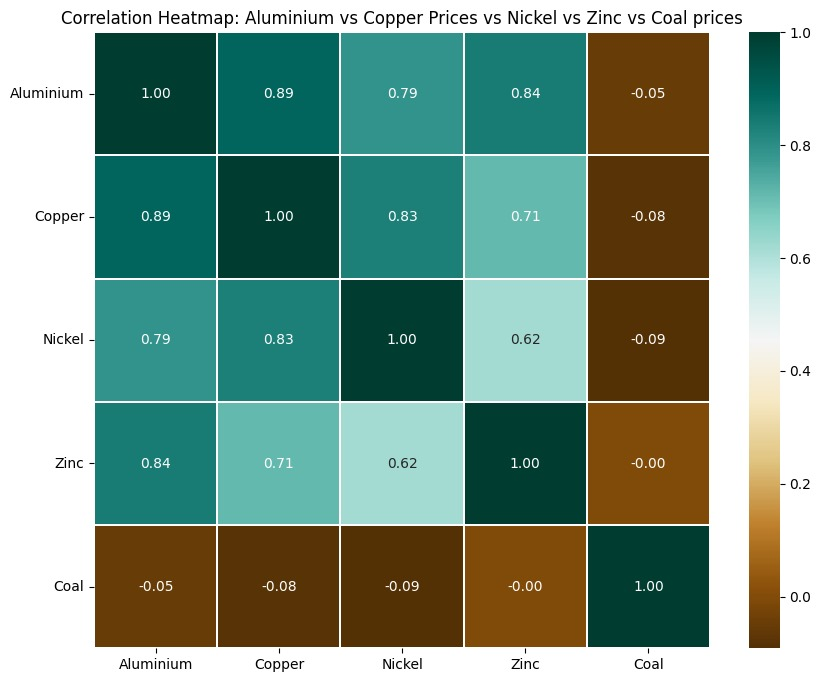
\includegraphics[width=12cm, height=10cm]{heatmap.jpeg}
		\caption{HeatMap}
		\label{fighm}
	\end{figure}
\end{center}

\begin{center}
	\begin{figure}[!htbp]
		\centering
		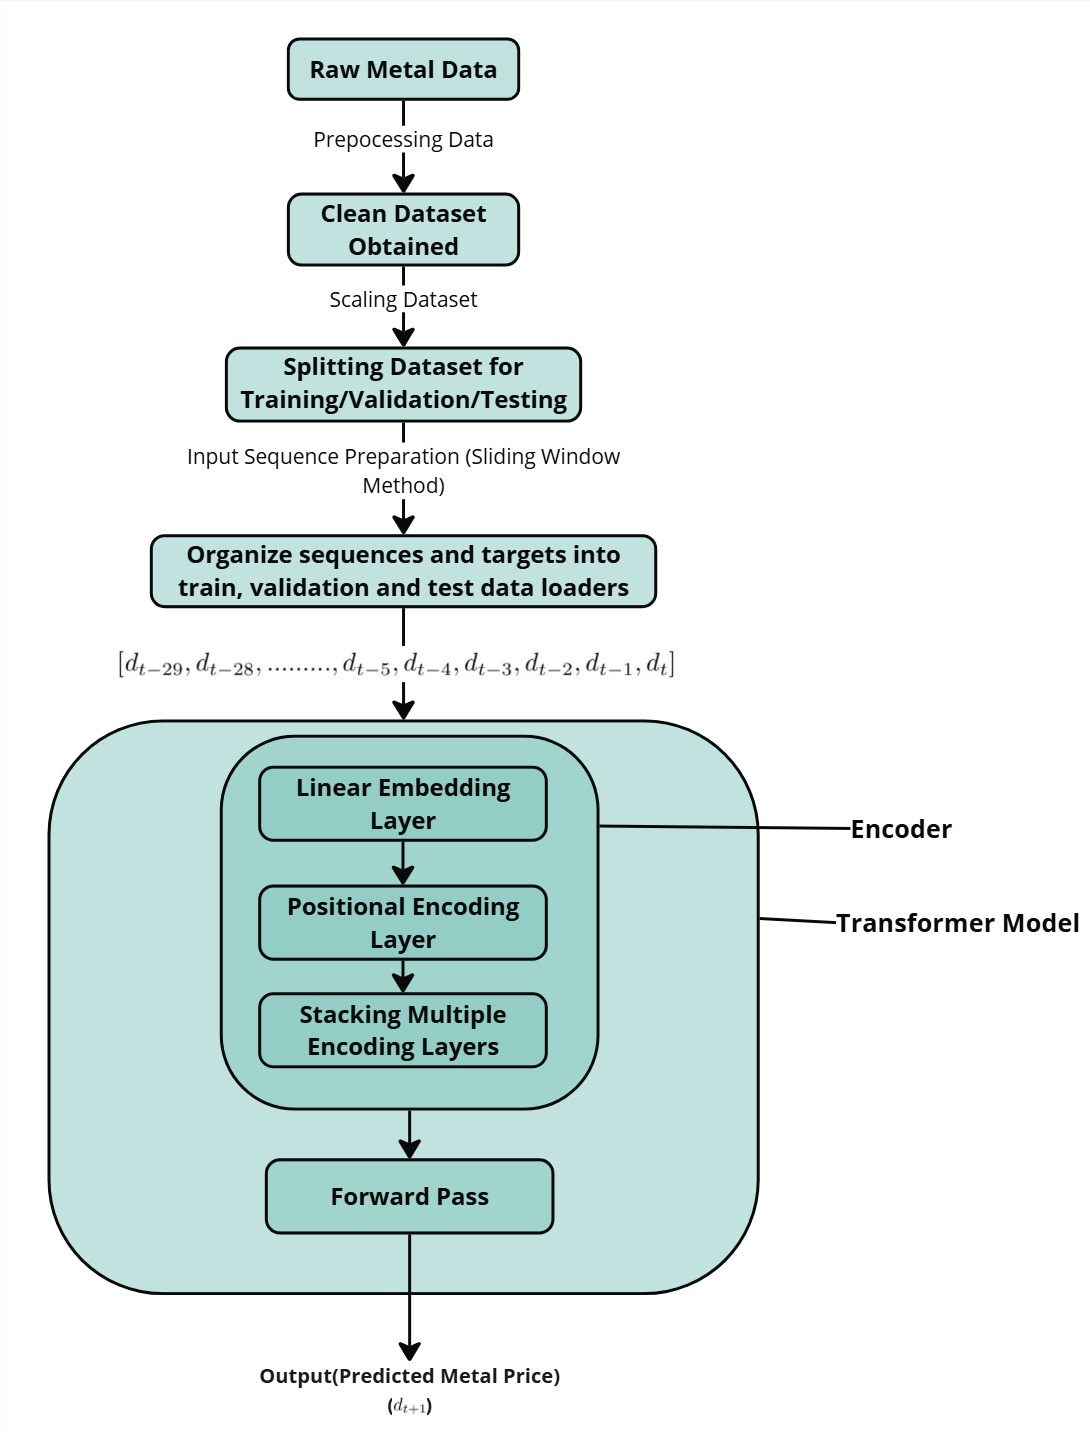
\includegraphics[width=11cm, height=15cm]{Transformer.jpg}
		\caption{Proposed System}
		\label{figpp}
	\end{figure}
\end{center}

\section{Experimentation}

\subsection{Experimental Data}
The global pricing of base metals such as Aluminium, Copper, Zinc, and others is determined by the London Metal Exchange, a renowned commodities exchange based in London, United Kingdom, established in 1877. The LME facilitates futures and options trading for various base and precious metals. Traders can engage in trading contracts for future delivery or options on a daily, weekly, and monthly basis. The prices of Aluminium, Copper, Zinc, and Nickel are denoted in US dollars per metric ton on the LME platform. In this work, we are interested in predicting the future price of the non-ferrous metal. Table \ref{tab1} presents the experimental data used in this work. Since metal price data is a time series, traditional random shuffling and splitting for cross-validation would disrupt the temporal dependencies. Therefore, we used the first continuous 70\% of the data for training, the next 20\% for validation, and the remaining 10\% for testing. Out of a total of 4171 days, 2920 days were allocated for training, 834 days for validation, and 417 days for testing. We acquired the experimental trading datasets for non-ferrous metals from the LME via Westmetall (https://www.westmetall.com/en/markdaten.php). Python was utilized for coding purposes. The code for both the proposed system and the baseline model is available in our GitHub repository at \textit{https://github.com/Nachiket1234/LME-Metal-Price-Prediction}.


\begin{table}
	\tbl{Experimental Data of non-ferrous Metal Prices from LME.}
	{\begin{tabular}{|p{2cm}|p{1cm}|p{2cm}|p{1.5cm}|p{2cm}|p{2cm}|} \hline
			\textbf{Stock Name} & \textbf{Time} & \textbf{Total Period} & \textbf{Training Period} & \textbf{Validation Period}& \textbf{Testing Period}\\ \hline 
			\multirow{2}{*}{Aluminium}&Start & 2008-01-02  &2008-01-02  &2019-07-18&2022-11-03 \\
			&End & 2024-07-01 &2019-07-17 &2022-11-02&2024-07-01\\ \hline
			\multirow{2}{*}{Copper}&Start & 2008-01-02  &2008-01-02  &2019-07-18&2022-11-03 \\
			&End  & 2024-07-01 &2019-07-17 &2022-11-02&2024-07-01\\ \hline
			\multirow{2}{*}{Zinc}&Start & 2008-01-02  &2008-01-02  &2019-07-18&2022-11-03 \\
			&End  & 2024-07-01 &2019-07-17 &2022-11-02&2024-07-01\\ \hline
			\multirow{2}{*}{Nickel}&Start & 2008-01-02  &2008-01-02  &2019-07-18&2022-11-03 \\
			&End  & 2024-07-01 &2019-07-17 &2022-11-02&2024-07-01\\ \hline
	\end{tabular}}
	\label{tab1}
\end{table}

Figure \ref{fig:A}, Figure \ref{fig:Co}, Figure \ref{fig:N}, Figure \ref{fig:Z} are the plots of the experimental datasets used in this work, it show the daily closing price of the stock.

\begin{center}
	\begin{figure}[!htbp]
		\centering
		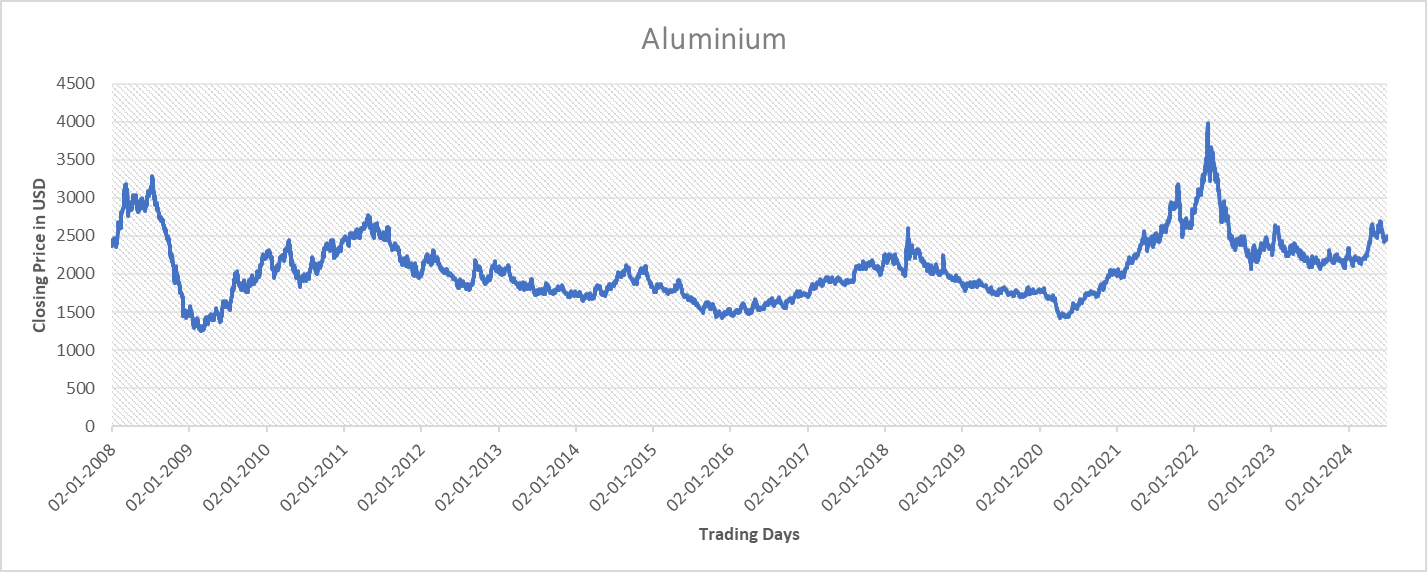
\includegraphics[width=13cm, height=7cm]{A.png}
		\caption{Daily close price series for Aluminium.}
		\label{fig:A}
	\end{figure}
\end{center}

\begin{center}
	\begin{figure}[!htbp]
		\centering
		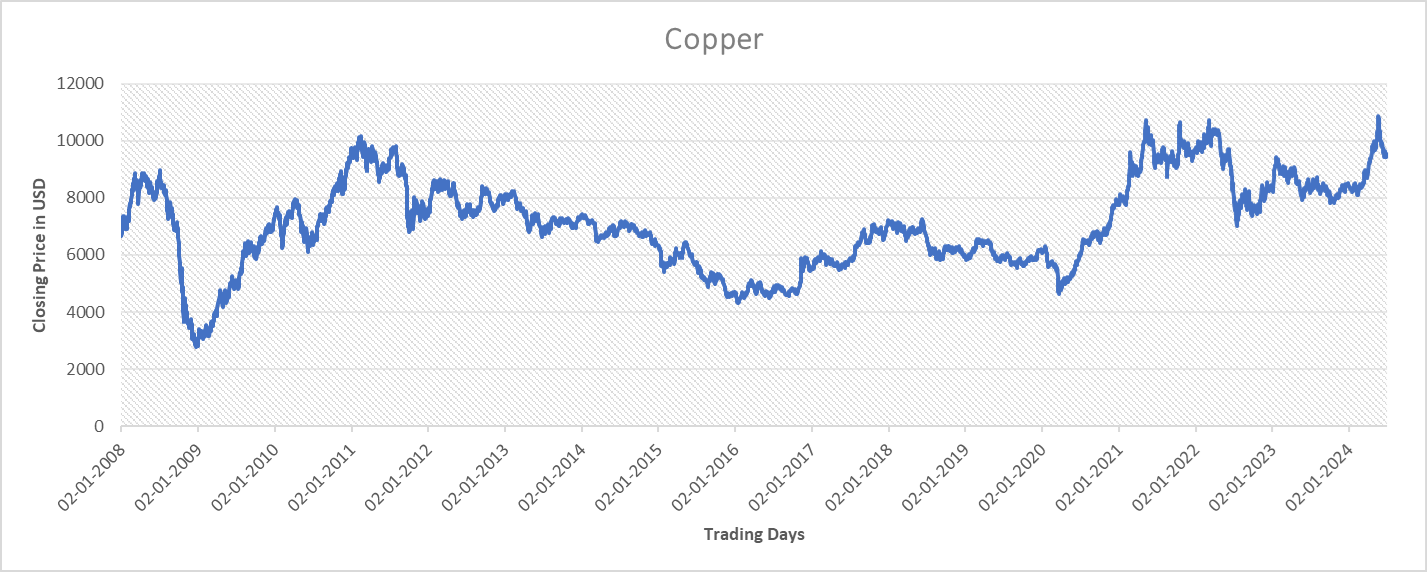
\includegraphics[width=13cm, height=7cm]{Co.png}
		\caption{Daily close price series for Copper.}
		\label{fig:Co}
	\end{figure}
\end{center}

\begin{center}
	\begin{figure}[!htbp]
		\centering
		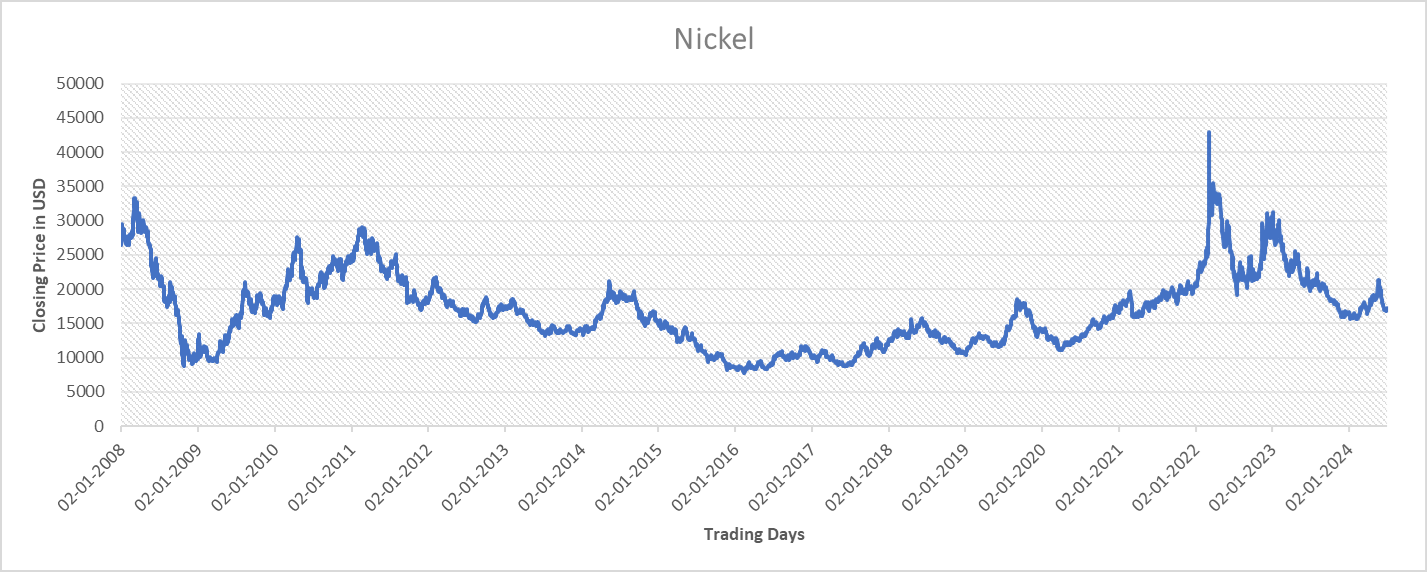
\includegraphics[width=13cm, height=7cm]{N.png}
		\caption{Daily close price series for Nickel.}
		\label{fig:N}
	\end{figure}
\end{center}

\begin{center}
	\begin{figure}[!htbp]
		\centering
		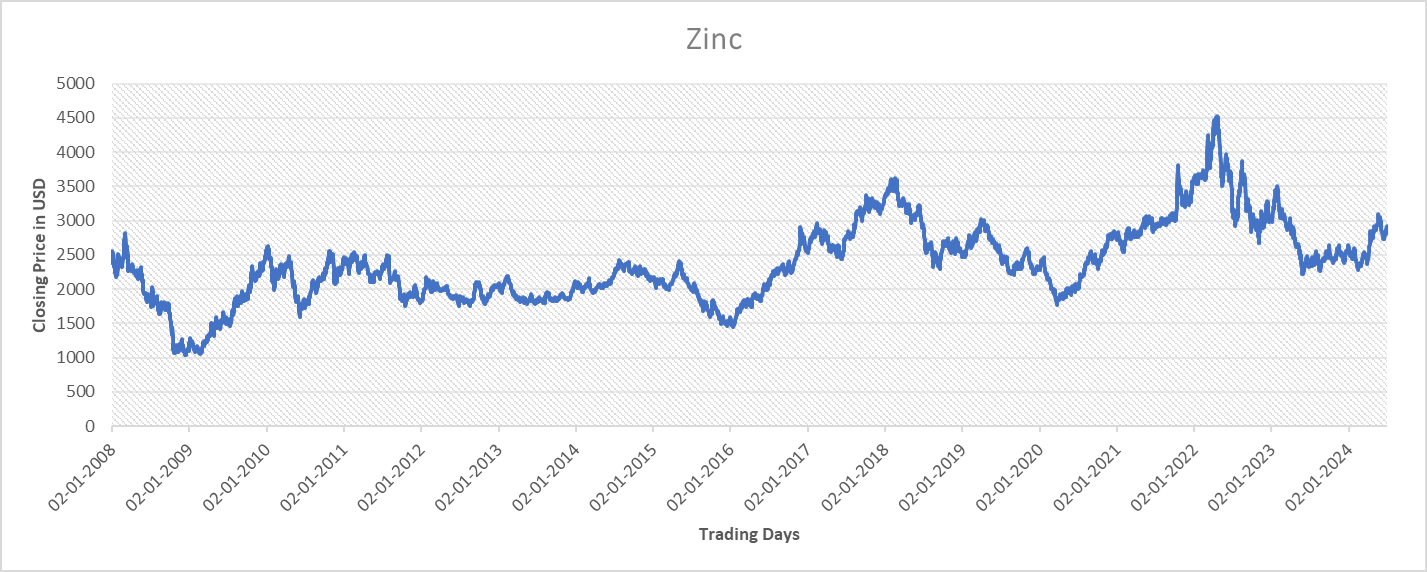
\includegraphics[width=13cm, height=7cm]{Z.png}
		\caption{Daily close price series for Zinc.}
		\label{fig:Z}
	\end{figure}
\end{center}

\subsection{Performance Evalution Measures}
Performance evaluation metrics are essential for assessing the effectiveness of models in various tasks, including regression problems. Mean Squared Error (MSE), Mean Absolute Error (MAE), and Mean Absolute Percentage Error (MAPE) are commonly used metrics for evaluating the performance of regression models.

\subsubsection{Mean Squared Error(MSE)}
A lower MSE indicates better model performance, and the metric is sensitive to outliers due to the squaring of errors.
\begin{equation}
	MSE = \frac{1}{n} \sum_{i=1}^{n} (y_i - \hat{y}_i)^2
\end{equation}

where:
\begin{align*}
	n & : \text{Number of data points} \\
	y_i & : \text{Actual value of the i-th data point} \\
	\hat{y}_i & : \text{Predicted value of the i-th data point}
\end{align*}

\subsubsection{Mean Absolute Error(MAE)}
Like MSE, a lower MAE indicates better model performance, and the metric is less sensitive to outliers than MSE.
\begin{equation}
	\text{MAE} = \frac{1}{n} \sum_{i=1}^{n} \lvert y_i - \hat{y}_i \rvert
\end{equation}

\subsubsection{Mean Absolute Percentage Error (MAPE)}
MAPE provides a percentage measure of the average relative error. A lower MAPE indicates better model performance, but it is sensitive to zero values in the actual data.
\begin{equation}
	MAPE = \frac{1}{n} \sum_{i=1}^{n} \left| \frac{y_i - \hat{y}_i}{y_i} \right| \times 100\%
\end{equation}

where:
\begin{align*}
	n & : \text{Number of data points} \\
	y_i & : \text{Actual value of the i-th data point} \\
	\hat{y}_i & : \text{Predicted value of the i-th data point}
\end{align*}

\section{Experimental Results}
We experimented with the proposed model on four non-ferrous metals viz Aluminium, Copper, Zink, and Nickel. We also compared the performance of the proposed model with the state-of-the-art sequential deep learning methods LSTM and GRU. Experimented with univariate and multivariate  LSTM and GRU. All models are trained and tested on the same dataset for fair comparison. The performance of the models is compared using the performance evaluation measures discussed in Section 5.2 on testing data only.

\par The experimental results of all models including the Transformer-based proposed model for experimental datasets of Aluminium, Copper, Zink, and Nickel are shown in the Table \ref{tab2},  \ref{tab3},  and \ref{tab4} in terms of MSE, MAE, and MAPE respectively. The proposed Transformer-based model outperformed all four baseline models on all four metals datasets with regards to MSE, MAE, and MAPE. 
\par The performance of all experimental models in terms of MSE on all experimental datasets is compared in Table \ref{tab2}, while Figure \ref{fig11} graphically depicts the same results. It is evident from both Table \ref{tab2} and Figure \ref{fig11} that the proposed model outperforms the baseline models in terms of MSE. Additionally, Table \ref{tab3} and Figure \ref{fig12} demonstrate the superiority of the proposed model in terms of MAE, while Table \ref{tab4} and Figure \ref{fig13} illustrate its superiority in terms of MAPE.

\begin{table}
	\tbl{Comparison of the performance of the five models, including the proposed Transformer-based model, across all four datasets in terms of Mean Squared Error.}
	{\begin{tabular}{|p{3cm}|p{2cm}|p{2cm}|p{2cm}|p{2cm}|} \hline
			\textbf{Model} & \textbf{Aluminum} & \textbf{Copper} & \textbf{Nickel} & \textbf{Zinc}\\ \hline 
			Transformer & 0.0001 & 0.0003 & 0.0002 & 0.0003\\ \hline 
			LSTM Multivariate & 0.0002 & 0.0004 & 0.0003 & 0.0004\\ \hline 
			GRU Multivariate & 0.0002 & 0.0005 & 0.0003 & 0.0004\\ \hline
			LSTM & 0.0003 & 0.0004 & 0.0004 & 0.0005\\ \hline
			GRU & 0.0003 & 0.0004 & 0.00035 & 0.0005\\ \hline
	\end{tabular}}
	\label{tab2}
\end{table}


\begin{table}
	\tbl{Comparison of the performance of the five models, including the proposed Transformer-based model, across all four datasets, evaluated in terms of Mean Absolute Error.}
	{\begin{tabular}{|p{3cm}|p{2cm}|p{2cm}|p{2cm}|p{2cm}|} \hline
			\textbf{Model} & \textbf{Aluminum} & \textbf{Copper} & \textbf{Nickel} & \textbf{Zinc}\\ \hline 
			Transformer & 0.01026 & 0.0132 & 0.01146 & 0.0143\\ \hline 
			LSTM Multivariate & 0.0114 & 0.0161 & 0.0121 & 0.0163\\ \hline 
			GRU Multivariate & 0.0122 & 0.0163 & 0.0125 & 0.0161\\ \hline
			LSTM & 0.0138 & 0.0174 & 0.0143 & 0.0181\\ \hline
			GRU & 0.0128 & 0.0161 & 0.0136 & 0.0178\\ \hline
	\end{tabular}}
	\label{tab3}
\end{table}



\begin{table}
	\tbl{Comparison of the performance of the five models, including the proposed Transformer-based model, across all four datasets in terms of Mean Absolute Percentage Error.}
	{\begin{tabular}{|p{3cm}|p{2cm}|p{2cm}|p{2cm}|p{2cm}|} \hline
			\textbf{Model} & \textbf{Aluminum} & \textbf{Copper} & \textbf{Nickel} & \textbf{Zinc}\\ \hline 
			Transformer & 2.65 & 1.80 & 2.88 & 2.99\\ \hline 
			LSTM Multivariate & 3.01 & 2.15 & 3.13 & 3.40\\ \hline 
			GRU Multivariate & 3.15 & 2.20 & 3.08 & 3.47\\ \hline
			LSTM & 3.64 & 2.41 & 3.83 & 3.87\\ \hline
			GRU & 3.29 & 2.18 & 3.58 & 3.72\\ \hline
	\end{tabular}}
	\label{tab4}
\end{table}

\begin{center}
	\begin{figure}[!htbp]
		\centering
		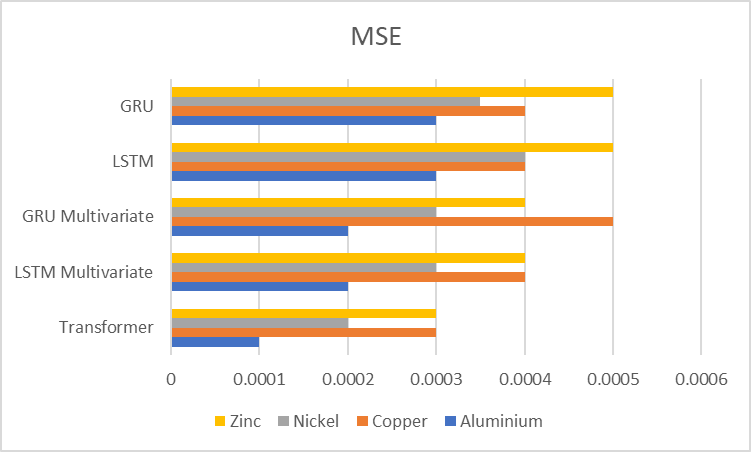
\includegraphics[width=15cm, height=7cm]{MSE.png}
		\caption{MSE of the five models including the proposed Transformer based model on testing datasets of four experimental metals.}
		\label{fig11}
	\end{figure}
\end{center}

\begin{center}
	\begin{figure}[!htbp]
		\centering
		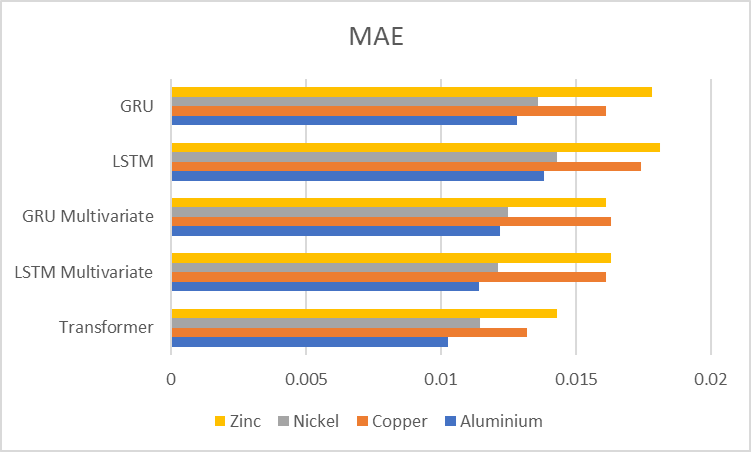
\includegraphics[width=15cm, height=7cm]{MAE.jpg}
		\caption{MAE of the five models including the proposed Transformer based model on testing datasets of four experimental metals.}
		\label{fig12}
	\end{figure}
\end{center}

\begin{center}
	\begin{figure}[!htbp]
		\centering
		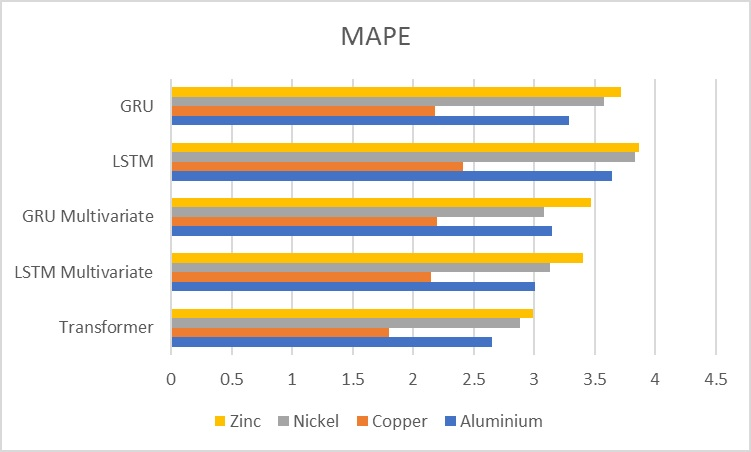
\includegraphics[width=15cm, height=7cm]{MAPE.png}
		\caption{MAPE of the five models including the proposed Transformer based model on testing datasets of four experimental metals.}
		\label{fig13}
	\end{figure}
\end{center}



\par To determine whether the experimental results are statistically significantly different, we performed a T-test. The T-test assesses whether there is a statistically significant difference between two groups. For a fair comparison, we evaluated the proposed model against univariate LSTM and GRU models, as the proposed Transformer-based model is also univariate in our case.

\par Table \ref{tab37} presents the Mean Squared Error (MSE) of the Proposed Model, the LSTM model, and the GRU model across four datasets. Table \ref{tab38} displays the results of the T-test comparisons between the Proposed Model and the LSTM model, as well as between the Proposed Model and the GRU model. In Table \ref{tab38}, the p-values are less than the significance level ($\alpha$) of 0.05, indicating that we reject the null hypothesis, which states that there is no significant difference between the group means. Therefore, the results of the Proposed Model compared to both the LSTM and GRU models are statistically significantly different. Similarly, Table \ref{tab40} shows comparable results for the same models on Mean Absolute Error (MAE) in Table \ref{tab39}.



\begin{table}
	\tbl{MSE on four metals by Proposed Model, LSTM and GRU}
	{\begin{tabular}{|p{3cm}|p{2cm}|p{2cm}|p{2cm}|} \hline
			\textbf{Metal Name} & \textbf{Proposed Model} & \textbf{LSTM} & \textbf{GRU}\\ \hline 
			Aluminium  & 0.0001 & 0.0003 & 0.0003\\ \hline 
			Copper  & 0.0003 & 0.0004 & 0.0004\\ \hline
			Nickel  & 0.0002 & 0.0004 & 0.00035\\ \hline
			Zinc  & 0.0003 & 0.0005 & 0.0005\\ \hline
	\end{tabular}}
	\label{tab37}
\end{table}




\begin{table}
	\tbl{Result of the T-test between different model's MSE.}
	{\begin{tabular}{|p{3cm}|p{3cm}|p{3cm}|} \hline
			\textbf{T-test matrix} & \textbf{Proposed Model and LSTM} & \textbf{LSTM and GRU} \\ \hline 
			t-Statistic  & -2.7815 & -2.5333 \\ \hline 
			p-Value  & 0.0319 & 0.0444 \\ \hline
			Significance Level($\alpha$)  & 0.005 & 0.005 \\ \hline
			
	\end{tabular}}
	\label{tab38}
\end{table}


\begin{table}
	\tbl{MAE on four metals by Proposed Model, LSTM and GRU}
	{\begin{tabular}{|p{3cm}|p{2cm}|p{2cm}|p{2cm}|} \hline
			\textbf{Metal Name} & \textbf{Proposed Model} & \textbf{LSTM} & \textbf{GRU}\\ \hline 
			Aluminium  & 0.01026 & 0.0138 & 0.0128\\ \hline 
			Copper  & 0.0132 & 0.0174 & 0.0161\\ \hline
			Nickel  & 0.01146 & 0.0143 & 0.0136\\ \hline
			Zinc  & 0.0143 & 0.0181 & 0.0178\\ \hline
	\end{tabular}}
	\label{tab39}
\end{table}


\begin{table}
	\tbl{Result of the T-test between different model's MAE.}
	{\begin{tabular}{|p{3cm}|p{3cm}|p{3cm}|} \hline
			\textbf{T-test matrix} & \textbf{Proposed Model and LSTM} & \textbf{LSTM and GRU} \\ \hline 
			t-Statistic  & -2.5560 & -2.2135 \\ \hline 
			p-Value  & 0.0431 & 0.0487 \\ \hline
			Significance Level($\alpha$)  & 0.005 & 0.005 \\ \hline
			
	\end{tabular}}
	\label{tab40}
\end{table}

\section{Conclusion}
Handling the long-term dependency on sequential data like metal price time series data is a problem of interest for industry and academia. LSTM results are better compared to RNN up to a certain extent. Recently deep learning model Transformer has shown significant performance improvement on sequential data. We proposed a model based on a Transformer to predict the future price of the non-ferrous metal using historical and current price time series data of the non-ferrous metal. Our experimental results on datasets of four non-ferrous metals viz Aluminium, Copper, Zink, and Nickel from LME conclude that the proposed model outperformed the baseline deep learning methods viz LSTM and GRU for sequential data. Till now Transformer for metal price prediction has not been studied. The main contribution of this research work is twofold. First, the use of a Transformer for non-ferrous metal price prediction. Second, is a comparison with the current state of art deep learning base model for sequential data with the proposed model. In the future, we would like to explore the Large Language Model for metal price prediction.  
\par Our experiment on the four datasets indicates that the Transformer-based model outperformed the LSTM and GRU-based models to predict future metal prices in terms of MSE, MAE, and MAPE.



\bibliographystyle{elsarticle-num}  % Use the style provided by Elsevier
\bibliography{references}          % Name of your .bib file (without the extension)

\end{document}

\endinput
%%
%% End of file `elsarticle-template-num.tex'.
